\documentclass[a4paper,oneside,11pt]{scrreprt}
\usepackage{scrhack} % to suppress warning

% include style from other file
\usepackage{style}

\begin{document}

\pagenumbering{gobble}

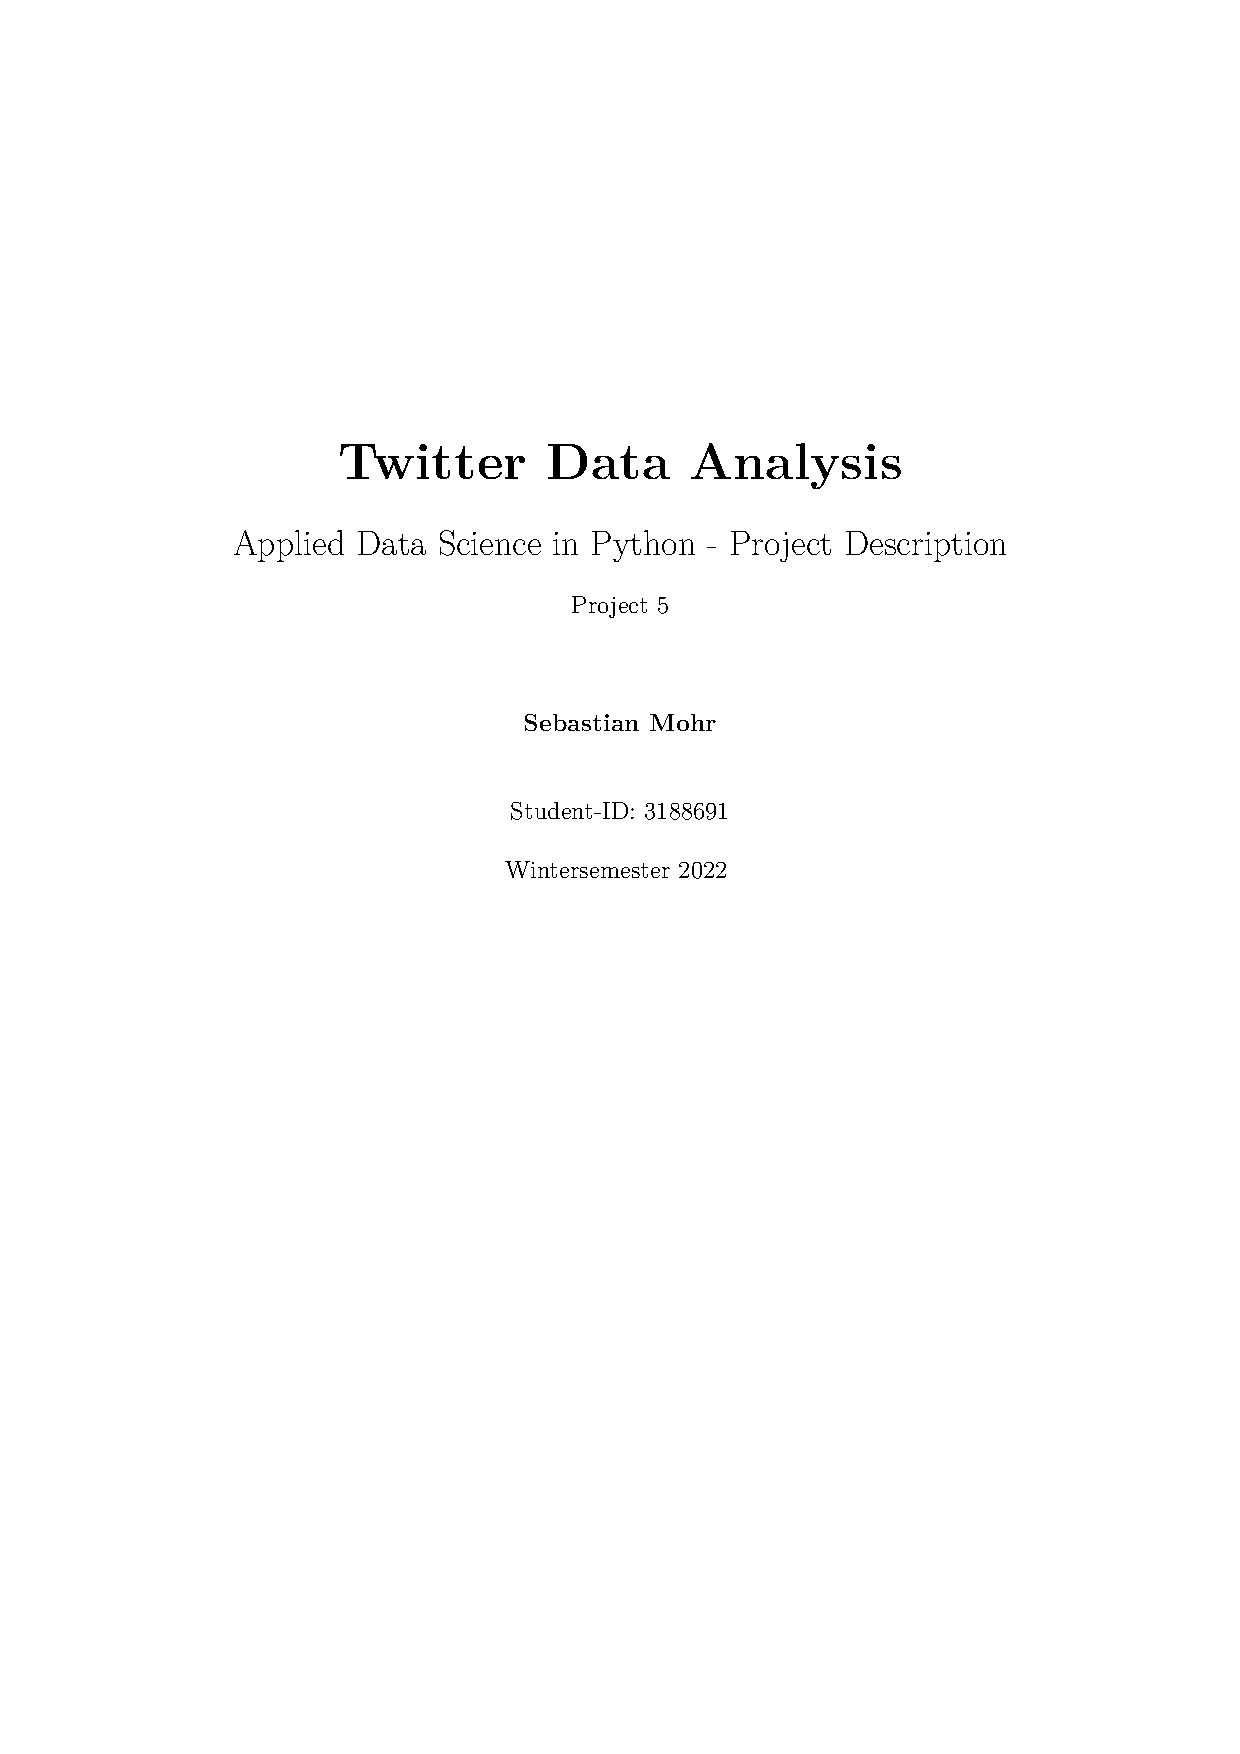
\includepdf{cover.pdf}

\newpage

\pagenumbering{arabic}

\chapter{How to solve the problem}

The goal of this project is to give users the ability to get information about a specific events hashtag and its top conversations on \requirement{Twitter}. The tweets for an event should be analyzed and the sentiment displayed for the user of the application. Additionaly the application shows the Top 10 hashtags and users associated with the chosen event. The user can further investigate the displayed data and look at the users, as well as their followers and the tweets.

\section{Getting the data}

The data that will be shown in the application will be gathered through the Twitter developer API. To achive this I signed up to Twitter with a new account that registered for the developer tools. Twitter already provides libraries for Python to easiely access its API.\\

First the app has to authenticate itself, to make sure that it is connected to the already created Twitter account. After the authentication the data can be gathered through a search url, that contains all the query parameters. Here the search url tells the API which data the application wants to get. The query parameters specify different metrics for the tweets, like the tweet author, date and time of its creation or used hashtags.\\

For this problem the API call will first retrieve all tweets that contain the hashtag of the searched for event. After analyzing the tweets, the the Top 10 contributors account data will also be retrieved from the API. 

\section{Data structuring}

The data provided by the Twitter API has to be processed somewhere in memory. To achive this goal, the data will be saved into objects of the \requirement{pandas} type \code{DataFrame}. \code{DataFrame}s have the advante of being able to store and filter large amounts of data in memory. Additionaly it can be easily exported to CSV. When saving the data on the hard drive it can be accessed every time when opening the application and only be updated when it is requested. This will boost the performance of the application, as it's not dependent on an internet connection for basic features and doesn't have to gather new data on every startup. The data can then still be updated in the background when clicking an update button for example. The application handles tweets and users, which will be saved in seperate \code{DataFrame}s.

\section{Tools and Application}

The backend of the application will be written in \code{Python}, as it provides good data analysing tools for the different problems of this project. To access the Twitter API I will use the \code{Tweepy} library. \code{Tweepy} provides several features to use all of the methods the Twitter API offers. For the \requirement{sentiment analysis} I will use the python library \code{TextBlob}. It's a text processing library which helps to analyze written text, which is perfect for analyzing many written tweets about a specific topic like a big event.\\

For the frontend I will use a web application, which will use several different \code{Type-} and \code{JavaScript} files. In these files I will build a User Interface with the library \code{React}. With \code{React} interactive web pages can be build that behave like a native running program would. To power \code{React} I will use \code{MUI} as the component library. 

\section{Modules and Algorithm}

The application will be split between front- and backend. In the frontend, only the user interface and basic computation, while the backend will handle all the Twitter API calls, as well as the data processing and persistence. \\

The application will firstly gather a specific number of tweets for the event from the Twitter API. After saving and analyzing the data, the Top 10 users by interactions will be figured out. Their info will also be retrieved from the Twitter API. After one of the Twitter users is clicked, its profile will be retrieved from Twitter and its followers and information will be displayed. The followers als can be viewed and their tweets will also be retrieved from the Twitter API.

\end{document}